%---------------------------------------------------------------------------------------------------------------------!Draft!-----------------------------------------------------------------------------------------------------------------
\subsection{Base da topologia de $X$ possui $i^*$ trivial para todos os elementos quando há recobrimento 1-conexo} %afirmação aqui significa teorema/proposição/colorário/lema
\label{pertence-a-base-se-e-somente-se-possui-i-trivial}
\begin{titlemize}{Lista de dependências}
	\item \hyperref[base-para-topologias-em-recobrimento-prop]{Base para as topologias em um recobrimento};\\ %'dependencia1' é o label onde o conceito Dependência 1 aparece (--à arrumar um padrão para referencias e labels--) 
	\item \hyperref[recobrimento-1-conexo-prop]{Existe recobrimento 1-conexo se e somente se X slsc};\\
    \item \hyperref[descrição-da-base-do-recobrimento-prop]{Descrição de $\tilde{\mathcal{B}}$ em termos de $X$};\\
    \item \hyperref[1-conexo-prop]{Propriedades de 1-conexo};\\
    \item \hyperref[levantamento-de-homotopia-prop]{Levantamento de Homotopia}
% quantas dependências forem necessárias.
\end{titlemize}
%Comentário sobre os objetos envolvidos na afirmação.
\begin{prop}% ou af(afirmação)/prop(proposição)/corol(corolário)/lemma(lema)/outros ambientes devem ser definidos no preambulo de Alg.Top-Wiki.tex 
	Sejam $p:E\rightarrow X$ um recobrimento 1-conexo e $U\subset X$ um aberto conexo por caminhos. Então $U\in \mathcal{B}$, onde $\mathcal{B}$ é base para a topologia de $E$ conforme definida em \ref{base-para-topologias-em-recobrimento-prop}, se se somente se $i_*:\pi_1(U,x)\rightarrow \pi_1(X,x)$ é trivial.\\

\end{prop}
\begin{dem}
    Por um lado, se $U\in \mathcal{B}$ temos que, dada a inclusão $i:U\rightarrow X$, $i_*:\pi(U,x)\rightarrow \pi(X,x)$ é um mapa trivial segundo argumentação realizada no início da demonstração do Teorema \ref{recobrimento-1-conexo-prop}.\newline

    Por outro lado, se $i_*:\pi_1(U,x)\rightarrow \pi_1(X,x)$ é trivial, vamos verificar que $U$ é uniformemente recoberto. Em particular, verifiquemos que $p^{-1}(U)=\underset{[\gamma]\in q^{-1}(X)}{\bigsqcup} \tilde{U}_{[\gamma]}$ onde $$\tilde{U}_{[\gamma]}=\{(\widetilde{\gamma*\eta})_{\tilde{x}}(1)|~\eta:I\rightarrow U,~\eta(0)=x\}$$, da mesma forma que é descrito no "caso 2" da Afirmação \ref{descrição-da-base-do-recobrimento-prop}. Isto é, $\tilde{U}_{[\gamma]}\in \tilde{B}$.

    Para tal, verifiquemos:

    \begin{enumerate}
        \item $\tilde{U}_{[\gamma]}\subset p^{-1}(U)$ para todo $[\gamma]$ pois
        $$p(\tilde{U}_{[\gamma]})=\{p((\widetilde{\gamma*\eta})_{\tilde{x}}(1))|~\eta:I\rightarrow U,~\eta(0)=x\}=$$$$=\{(\gamma*\eta)(1)|~\eta:I\rightarrow U,~\eta(0)=x\}=\{\eta(1)\in U|~\eta:I\rightarrow U,~\eta(0)=x\}\subset U$$\newline

        \item $p^{-1}(U)\subset \underset{[\gamma]\in q^{-1}(x)}{\bigcup} \tilde{U}_{[\gamma]}$

        Seja $\tilde{y}\in p^{-1}(U)$, seja $\eta:I\rightarrow U$ com $\eta(0)=x$ e $\eta(1)=y=p(\tilde{y})$ e seja $\tilde{x}=\tilde{\overline{\eta}}_{\tilde{y}}(1)$, de forma que $p(\tilde{x})=x$.

        Seja $ \xi:I\rightarrow E$ com $\xi(0)=e_0$, $\xi(1)=\tilde{x}$ e seja $\gamma=p\circ \xi$. Então $ \tilde{y}\in \tilde{U}_{[\gamma]}$ pois $(\widetilde{\gamma * \eta})_{e_0}(1)=\tilde{\eta}_{\tilde{x}}(1)=\tilde{y}$.\newline

        \item Se $[\gamma_0]\neq [\gamma_1]\in q^{-1}(x)$, então $ \tilde{U}_{[\gamma_0]}\cap \tilde{U}_{[\gamma_1]}=\emptyset$

        Suponha que $\tilde{y}\in \tilde{U}_{[\gamma_0]}\cap\tilde{U}_{[\gamma_1]}$. Sejam $\eta_0, \eta_1: I\rightarrow U$ curvas tais que $(\widetilde{\gamma_0*\eta_0})_{e_0}(1)=(\widetilde{\gamma_1*\eta_1})_{e_0}(1)=\tilde{y}$, como representado na figura \ref{fig:classes-distintas-de-curvas} a seguir.

\begin{figure}[h!]
         \centering
         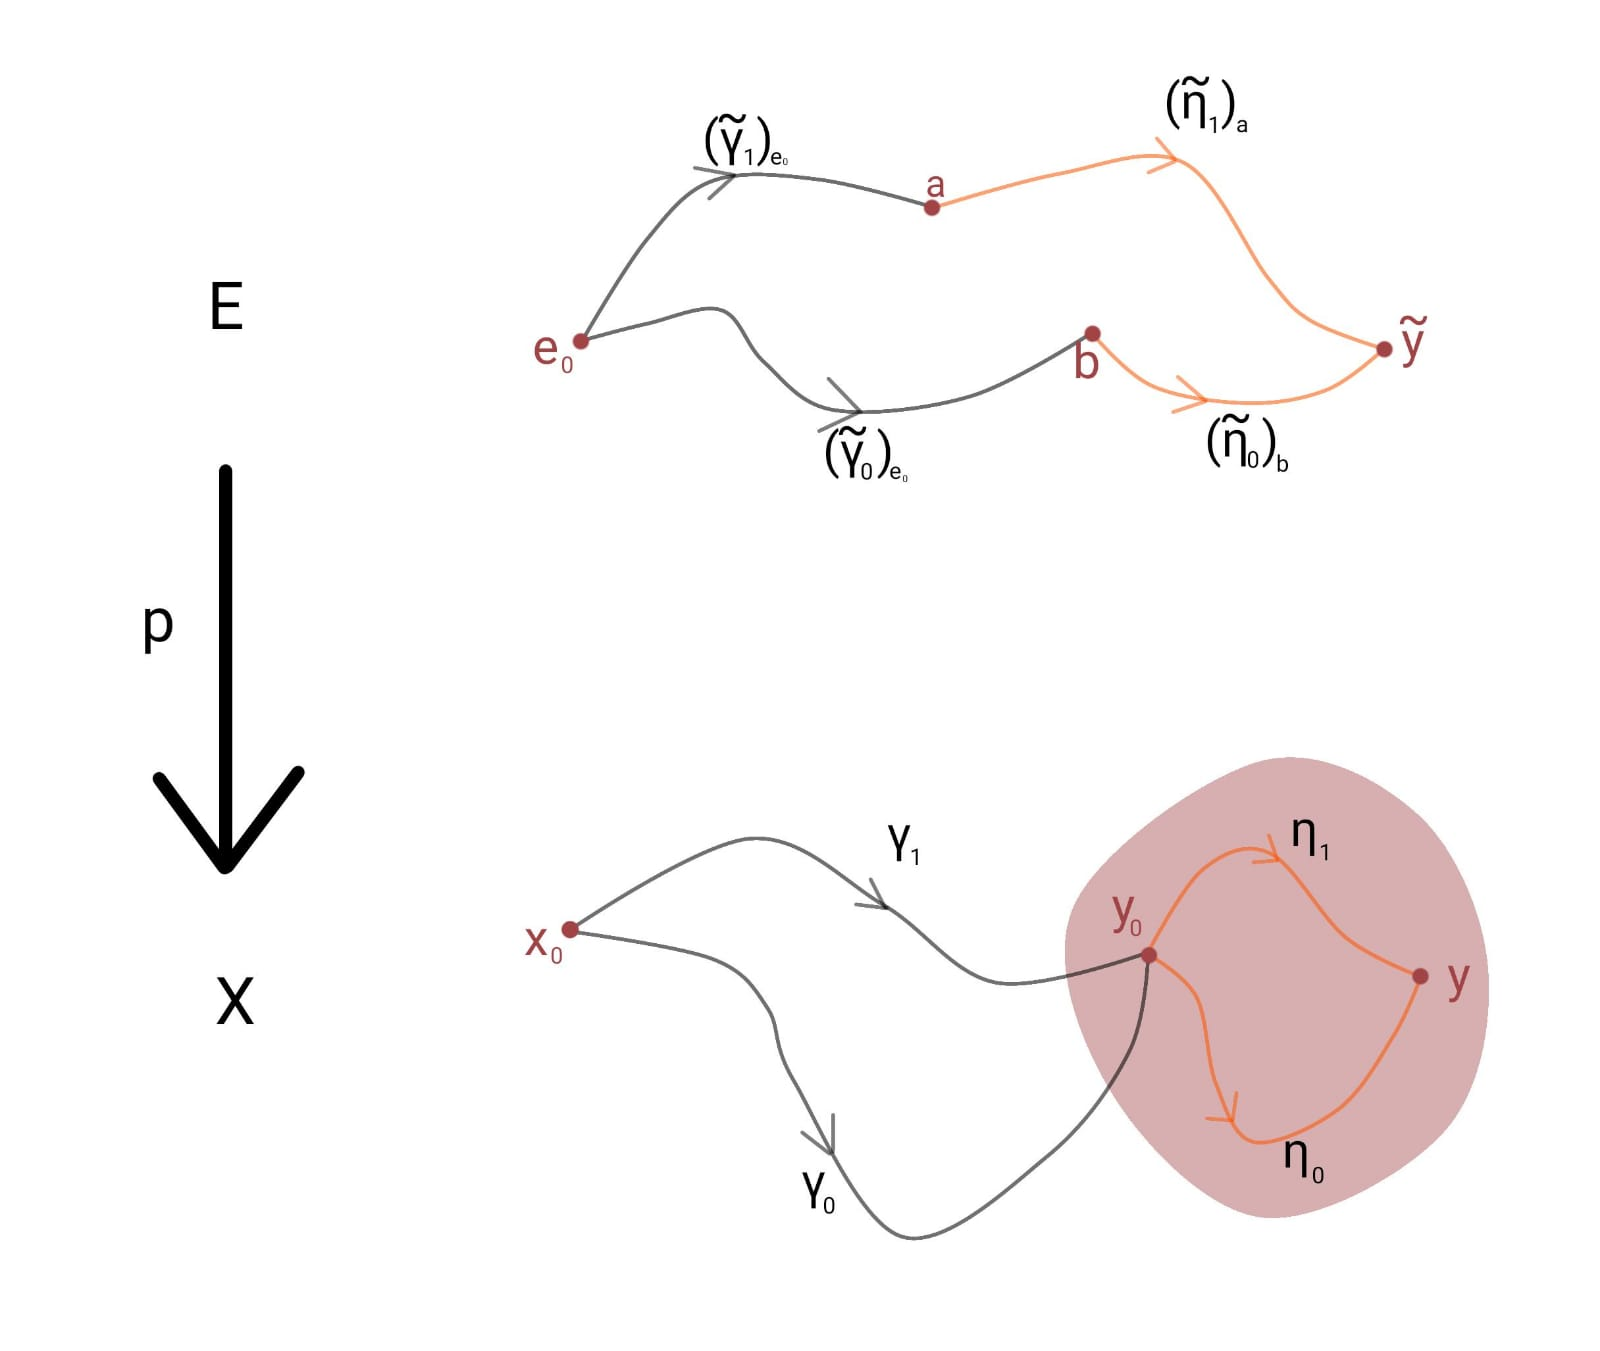
\includegraphics[width=0.8\linewidth]{conteudo/fig-classes-distintas-de-curvas.jpeg}
         \caption{Classes distintas de curvas, mas $\tilde{y}$ na intersecção dos abertos}
         \label{fig:classes-distintas-de-curvas}
     \end{figure} 

        
        Assim, temos que $p\circ(\widetilde{\gamma_0*\eta_0})_{e_0}(1)=y=p\circ(\widetilde{\gamma_1*\eta_1})_{e_0}(1)$ e portanto $\eta_0(1)=y=\eta_1(1)$.

        Na mesma figura, é possível notar que $\eta_0*\overline{\eta}_1$ é um laço em $U$ com ponto base $y$. Como nos foi dado que $i^*:\pi(U,x)\rightarrow \pi_1(X,x)$ é trivial e $U$ conexo por caminhos, temos que

        $$(\eta_0*\overline{\eta}_1)\sim c_y~(\text{rel}~\partial I) \Rightarrow (\widetilde{\eta_0 * \overline{\eta_1}})_{\tilde{y}}\sim  c_{\tilde{y}}~(\text{rel}~\partial I)\Rightarrow (\tilde{\gamma}_0)_{e_0}(1)=(\tilde{\gamma}_1)_{e_0}(1),$$ diferentemente do que a imagem indica.

        Como $E$ é 1-conexo, utilizando a Proposição \ref{1-conexo-prop} concluí-se que $[\gamma_0]=[\gamma_1]$, um absurdo por contradizer a hipótese inicial.\newline
        

    
        \item A restrição $p|_{\tilde{U}_{[\gamma]}}:\tilde{U}_{[\gamma]}\rightarrow U $ é bijeção

        Para verificar a sobrejetividade basta notar que para todo $y\in U$ é possível tomar a curva $\eta:I\rightarrow U$ tal que $\eta(0)=x$ e $\eta(1)=y$. Temos que se $\tilde{y}=(\widetilde{\gamma*\eta})_{e_0}(1)\in \tilde{U}_{[\gamma]}$, então $p(\tilde{y})=y$, como queríamos.

        Para a verificação da injetividade, basta supor que $p((\widetilde{\gamma*\eta_0})_{e_0}(1))=p((\widetilde{\gamma*\eta_1})_{e_0}(1))$ onde $\eta_0, \eta_1:I\rightarrow U$ são tais que $\eta_0(0)=x=\eta_1(0)$ e $\eta_0(1)=\eta_1(1)$. Portanto, $\eta_0*\overline{\eta}_1$ é laço e assim $\eta_0\sim \eta_1~(\text{rel }\partial I)$.
        Isso significa que, se $\tilde{x}=\tilde{\gamma}_{e_0}(1)$, então $(\tilde{\eta}_0)_{\tilde{x}}(1)= (\tilde{\eta}_1)_{\tilde{x}}(1)$ segundo Corolário presente em \ref{levantamento-de-homotopia-prop}. Assim, $(\widetilde{\gamma*\eta_0})_{e_0}(1)=(\gamma*\eta_1)_{e_0}(1)$.\newline

        \item A restrição $p|_{\tilde{U}_{[\gamma]}}$ é aplicação aberta pois $\tilde{U}_{[\gamma]}\in \tilde{\mathcal{B}}$ é uma placa do recobrimento.\newline
    \end{enumerate}

    Assim, verificamos que $U$ é uniformemente recoberto, isto é, $U \in \mathcal{B}$ como queríamos.\newline
\end{dem}

O resultado acima implica que a base $\mathcal{B}$ pode ser descrita como $\mathcal{B}=\{U\subset X|~U\text{ é conexo por caminhos e }i_*:\pi_1(U,x)\rightarrow \pi_1(X,x)\text{ é trivial}\}$

%\begin{titlemize}{Lista de consequências}
%	\item \hyperref[consequencia1]{Consequência 1};\\ %'consequencia1' é o label onde o conceito Consequência 1 aparece
%	\item \hyperref[]{}
%\end{titlemize}

%[Bianca]: Um arquivo tex pode ter mais de uma afirmação (ou definição, ou exemplo), mas nesse caso cada afirmação deve ter seu próprio label. Dar preferência para agrupar afirmações que dependam entre sí de maneira próxima (um teorema e seu corolário, por exemplo)
